% !TeX program = uplatex
\documentclass[uplatex, a4j, dvipdfmx]{jsarticle}

% ===================================================================
% ▼ プリアンブル(各種設定) ▼
% ===================================================================

% --- ページレイアウト設定 ---
\usepackage[left=25mm, right=25mm, top=30mm, bottom=30mm]{geometry}

% --- 基本機能パッケージ ---
\usepackage{graphicx}      % 画像ファイルを読み込む
\usepackage{pdfpages}      % PDFファイルを読み込む
\usepackage{enumitem}      % 箇条書きのカスタマイズ
\usepackage{makecell}      % 表のセル内で改行する
\usepackage[T1]{fontenc}   % フォントエンコーディングの指定
\usepackage{url}           % urlを記述できるようにする
\usepackage{subcaption}    % 図をグループ化するために追加

% --- 日本語環境設定 ---
\usepackage{plext}         % 日本語組版の拡張機能
\usepackage{okumacro}      % 奥村氏作成のマクロ集
\usepackage[deluxe]{otf}   % 日本語フォント設定

% --- 数式・フォント関連パッケージ ---
\usepackage{amsmath}              % 高度な数式環境を提供 (必須)
\usepackage{newtxtext, newtxmath} % 本文と数式のフォントをTimes系に変更
\usepackage{siunitx}              % 単位(SI単位系)を扱う

% --- グラフィックス・作図関連パッケージ ---
\usepackage{tikz}                 % 高機能な作図ツール
\usepackage{circuitikz}           % 電気回路図の描画
\usetikzlibrary{circuits.logic.US} % 論理回路のライブラリ
\usepackage{tabularray}           % 高機能な表作成ツール

% --- 文書デザイン関連パッケージ ---
\renewcommand{\headfont}{\mcfamily} % ページ番号のフォント
\usepackage{titlesec}               % 見出しのスタイルをカスタマイズ
\titleformat{\section}{\normalfont\Large\bfseries}{\thesection}{1em}{}
\titleformat{\subsection}{\normalfont\large\bfseries}{\thesubsection}{1em}{}
\titleformat{\subsubsection}{\normalfont\normalsize\bfseries}{\thesubsubsection}{1em}{}
\usepackage{fancyhdr}               % ヘッダー・フッターのカスタマイズ
\pagestyle{fancy}
\fancyhead{}
\fancyfoot{}
\fancyfoot[C]{\thepage}
\renewcommand{\headrulewidth}{0pt}
\renewcommand{\footrulewidth}{0pt}

% --- 警告抑制パッケージ ---
\usepackage{silence}
\WarningFilter{caption}{Unknown document class (or package)}
\WarningFilter{latexfont}{Some font shapes}
\WarningFilter{latexfont}{Font shape}

% --- 本文全体のフォントサイズ・行間の設定 ---
\AtBeginDocument{%
  \fontsize{10.5pt}{15pt}\selectfont
}

% ===================================================================
% ▼ 本文ここから ▼
% ===================================================================

\begin{document}

\pagestyle{empty}
\includepdf[pages=-, fitpaper=true]{cover.pdf}

\setcounter{page}{1}
\pagestyle{fancy}

\section{目的}
本実験の目的は、実験室での測定を通して、以下の2点を理解することである。加えて、これらの測定に必要となる機器の使い方や原理を理解することも目的とする。
\begin{itemize}
    \item AND回路に代表される論理素子が、信号を入力から出力に伝えるときに生じる遅延
    \item ディジタル回路において値を記憶するための回路構成
\end{itemize}

\section{オシロスコープと信号発生装置}
\subsection{原理}
\subsubsection{信号発生器}
信号発生器は、様々な波形の周期的な電圧信号を出力することができる機器であり、ファンクションジェネレータ(function generator)とも呼ばれる。
正弦波、方形波、三角波、のこぎり波といった基本的な波形に加えて、機器によってはこれらを組み合わせた任意波形を出力できるものもある。
信号発生器は、通常、電気計測器に分類されるが、信号発生器だけで計測をするのではなく、計測対象の電気回路や電子回路に電圧信号を与える役割を担う。

\subsubsection{オシロスコープ}
オシロスコープ(oscilloscope)とは、横軸を時間、縦軸を電圧値として、信号の波形を描く装置である。
入力電圧をトランジスタ等の電子回路で処理することによって波形描画するアナログ型と、入力電圧をディジタル値に変換してからディジタル回路で処理するディジタル型に大別される。
現在は、ディジタル型のオシロスコープが主流であり、実験で用いるものもディジタル型である。

オシロスコープでは、プローブ(probe)と呼ばれる器具を使って、測定対象物とオシロスコープを接続する。
プローブは、通常のリード線と異なって、高周波の電圧波形を測定できるよう精密に作られている。
特に、強い曲げによって故障する可能性があるため、取扱いには注意が必要である。
プローブは、針状の端子とワニ口クリップ状の端子の2端子を持っている。
前者を測定対象の電圧に接続し、後者は基準電位(グラウンド)に接続する。

\subsection{使用機器}
\noindent
信号発生器 SIGLENT Technologies社 SDG1032X, オシロスコープ Tektronix社 TBS1052C,
抵抗器(\SI{10}{\kilo\ohm} 2個), ブレッドボード

\subsection{実験方法}
以下の各実験では、プローブの減衰率を「x10」とし、かつ、オシロスコープの「工場出荷時設定」のボタンを押して初期状態としてから始めた。

\subsubsection*{実験1-1 オシロスコープと信号発生器の基本的な使用方法}
ブレッドボード上で図\ref{E1}の回路を作成し、電圧$v_1$をオシロスコープに表示しながら信号発生器を操作して、周波数\SI{1}{\kilo\hertz}、振幅\SI{5}{\volt}(\text{P-P}値\SI{10}{\volt})に調整し、そのときに信号発生器で出力している\text{P-P}値を記録した。
その状態で、オシロスコープに電圧$v_1$,$v_2$を表示させた。
実験で用いた抵抗器の抵抗値を、ディジタルマルチメータで測定すると、どちらも\SI{9.94}{\kilo\ohm}と分かった。
このときオシロスコープで観測された電圧$v_1$と$v_2$の波形を各電圧の\SI{0}{\volt}レベルが画面の中心になるように調整したものを、図\ref{O1}に示す。

図\ref{O1}より、\text{P-P}値は\SI{9.920}{\volt}だと分かる。
また、$v_2$の\text{P-P}値が\SI{4.960}{\volt}であることから、正しく分圧できていると分かる。
\begin{figure}[htbp]
    \centering
    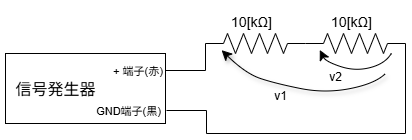
\includegraphics[width=0.7\linewidth]{picture/E1.png}
    \caption{実験回路1}
    \label{E1}
\end{figure}

\begin{figure}[htbp]
    \centering
    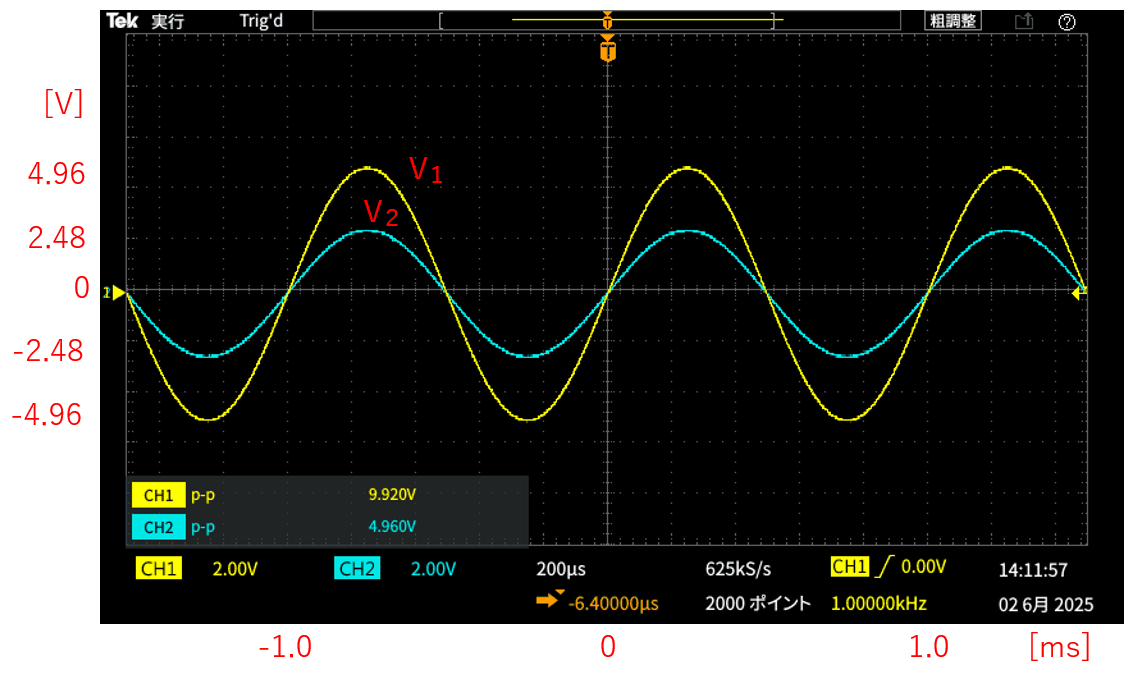
\includegraphics[width=0.8\linewidth]{picture/O1.png}
    \caption{電圧$v_1$,$v_2$の波形}
    \label{O1}
\end{figure}

この後の実験1-2は、信号発生器の出力を変化させずに行うため、信号発生器の出力電圧は変更せずに使用した。

\subsubsection*{実験1-2 信号発生器の出力電圧と内部抵抗}
実験1-1から出力電圧は変化させずに、信号発生器の出力を回路から外した状態で、信号発生器の出力電圧をオシロスコープで測定して、\text{P-P}値を求めた。

図\ref{O2}より、\text{P-P}値は\SI{9.920}{\volt}だと分かる。
このことから、信号発生器から\SI{9.920}{\volt}の電圧がかけられていると分かる。

この実験が終了した後、信号発生器の出力を回路につないで、実験1-1の最後の状態に戻した。

\begin{figure}[htbp]
    \centering
    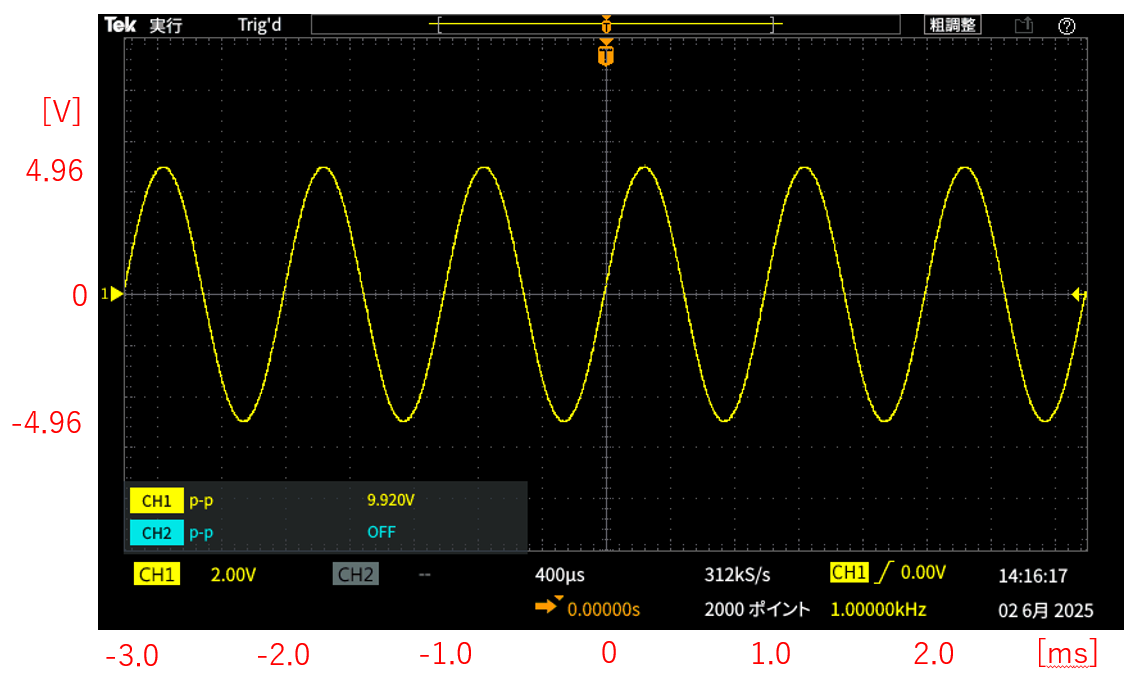
\includegraphics[width=0.8\linewidth]{picture/O2.png}
    \caption{信号発生器の出力電圧の波形}
    \label{O2}
\end{figure}

\subsubsection*{実験1-3 各種波形の出力}
実験1-1と同じ回路において電圧$v_1$をオシロスコープで表示し、以下の波形が表示されるように信号発生器を操作した。
\begin{enumerate}[label=(\arabic*)]
    \item 周波数\SI{1}{\kilo\hertz}、実効値\SI{5}{\volt}の正弦波
    \item 周波数\SI{1}{\kilo\hertz}、振幅\SI{5}{\volt}の正弦波に\SI{5}{\volt}のバイアスをかけて、最小値\SI{0}{\volt}、最大値\SI{10}{\volt}とした波形
    \item 周波数\SI{10}{\kilo\hertz}、最小値\SI{-5}{\volt}、最大値\SI{5}{\volt}の三角波
    \item 周波数\SI{10}{\kilo\hertz}、最小値\SI{0}{\volt}、最大値\SI{5}{\volt}の方形波
\end{enumerate}
それぞれの波形について、波形画像を保存したものを図\ref{O3-6}に示す。

\begin{figure}[htbp]
    \centering
    \begin{subfigure}[b]{0.48\textwidth}
        \centering
        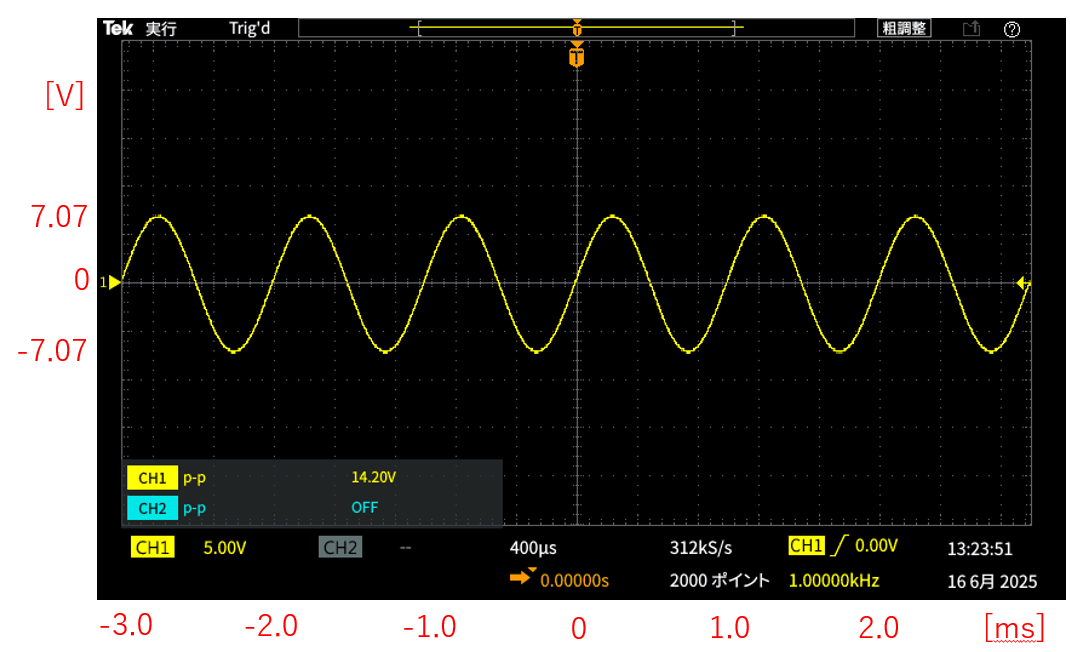
\includegraphics[width=\linewidth]{picture/O3.png}
        \caption{(1)の条件での波形}
        \label{O3}
    \end{subfigure}
    \hfill
    \begin{subfigure}[b]{0.48\textwidth}
        \centering
        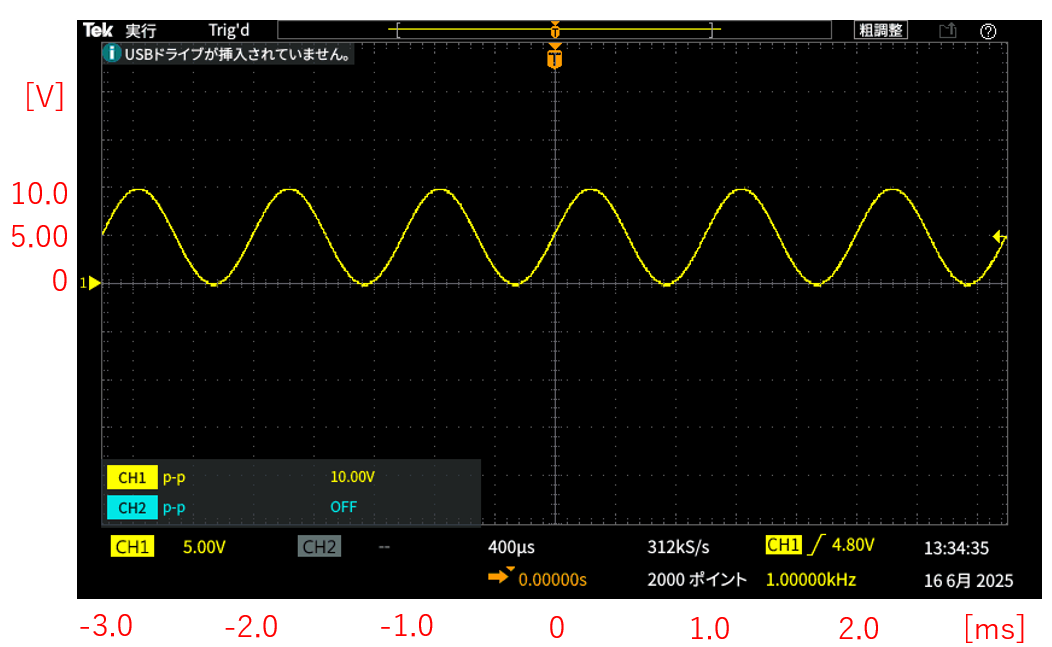
\includegraphics[width=\linewidth]{picture/O4.png}
        \caption{(2)の条件での波形}
        \label{O4}
    \end{subfigure}
    
    \vspace{1ex}
    
    \begin{subfigure}[b]{0.48\textwidth}
        \centering
        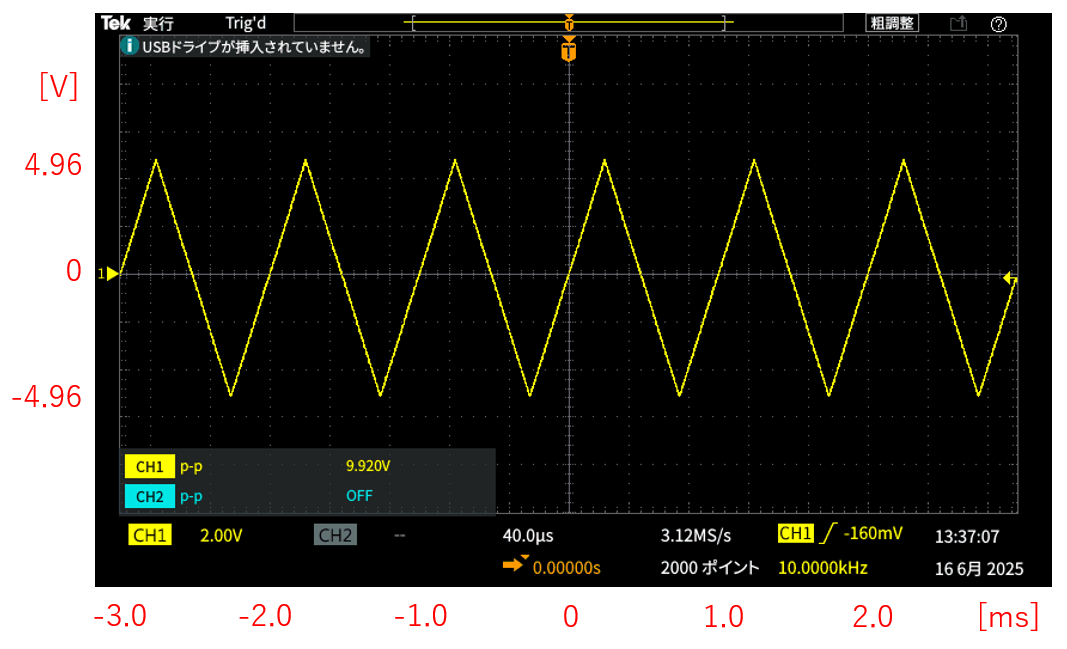
\includegraphics[width=\linewidth]{picture/O5.png}
        \caption{(3)の条件での波形}
        \label{O5}
    \end{subfigure}
    \hfill
    \begin{subfigure}[b]{0.48\textwidth}
        \centering
        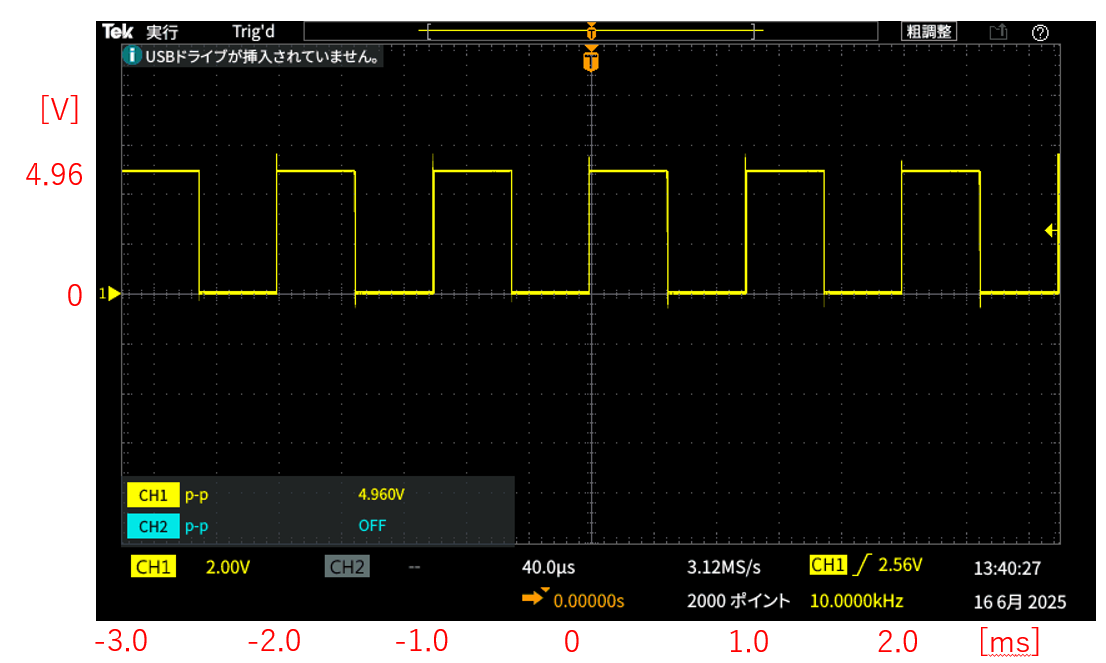
\includegraphics[width=\linewidth]{picture/O6.png}
        \caption{(4)の条件での波形}
        \label{O6}
    \end{subfigure}
    \caption{実験1-3 各種波形の出力結果}
    \label{O3-6}
\end{figure}

\subsubsection*{実験1-4 ACモードとDCモード}
この実験は、実験1-3の方形波を出力した状態で行った。
オシロスコープをDCモードとACモードに設定して、それぞれの場合の波形画像を保存した。
以下に、保存した波形画像を図\ref{O7-8}に示す。

\begin{figure}[htbp]
    \centering
    \begin{subfigure}[b]{0.48\textwidth}
        \centering
        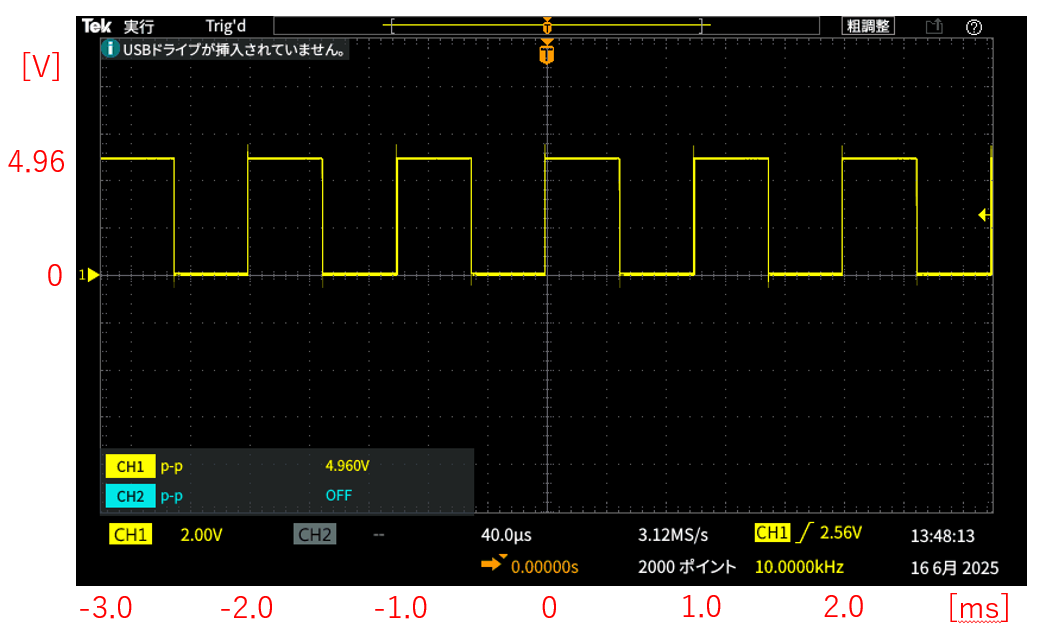
\includegraphics[width=\linewidth]{picture/O7.png}
        \caption{DCモードでの波形}
        \label{O7}
    \end{subfigure}
    \hfill
    \begin{subfigure}[b]{0.48\textwidth}
        \centering
        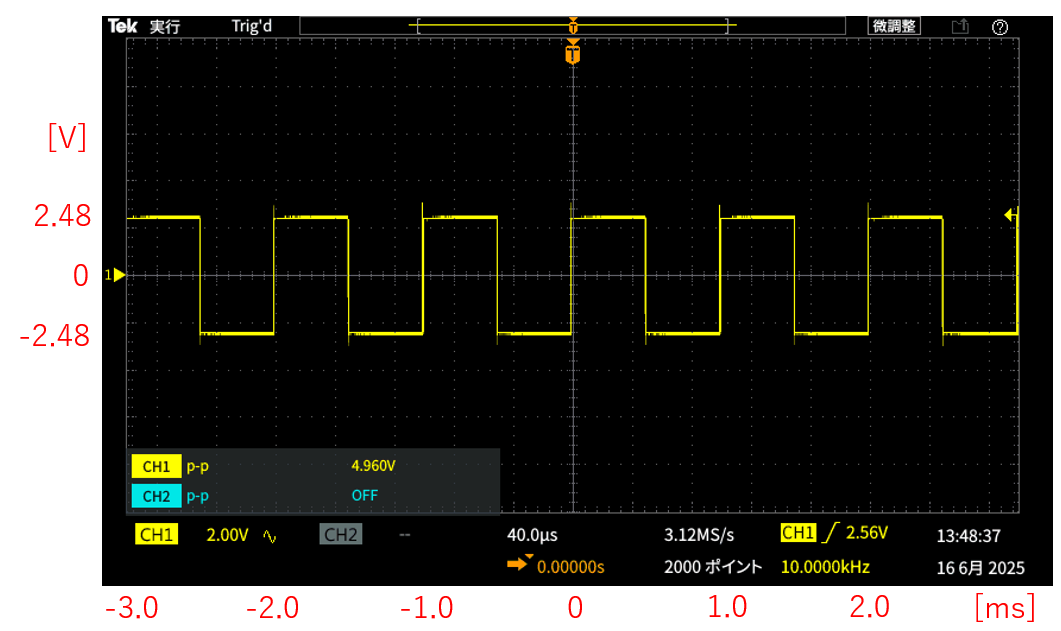
\includegraphics[width=\linewidth]{picture/O8.png}
        \caption{ACモードでの波形}
        \label{O8}
    \end{subfigure}
    \caption{実験1-4 AC/DCモードの波形}
    \label{O7-8}
\end{figure}

\clearpage

\subsection{考察課題}
\begin{enumerate}[label=(\arabic*), itemsep=1.5ex, leftmargin=2.5em]
    \item 実験1-1の電圧$v_1$と実験1-2は、どちらも$P-P$値が\SI{9.92}{\volt}だったが、本来異なる電圧値が測定される。なぜなら、実験1-1の場合は図\ref{E1}の回路に電流が流れるため、信号発生器の内部抵抗によって電圧降下が起きるのに対し、実験1-2の場合は信号発生器の出力端子が解放されているため、電圧降下が起きないためである。そのため、実験1-1の$P-P$値は実験1-2の$P-P$値よりも低くなる。

    実験1-1の電圧$v_1$と実験1-2の$P-P$値が等しくなった理由は、微小な電圧の変化をオシロスコープが識別できなかったからではないかと考えた。
    
    \item プローブの減衰率について、通常、「x1」ではなく、「x10」が使用される。なぜなら、「x1」プローブは内部抵抗なしに入力インピーダンスを直接回路につなげるのに対し、「x10」プローブは内部抵抗\SI{9}{\mega\ohm}の抵抗を持っているためである。オシロスコープの入力インピーダンスは\SI{1}{\mega\ohm}のため、「x1」プローブと「x10」プローブ使用時では、測定系全体のインピーダンスが10倍違うこととなる。そのため、「x10」を使用することで、測定対象の回路への影響を低減でき、より正確な値が測定できるためである。
    
    \item 実験1-4で得られた図\ref{O7-8}より、DCモードでの波形は\SI{0}{\volt}から\SI{4.96}{\volt}の範囲であるのに対し、ACモードでの波形は\SI{-2.48}{\volt}から\SI{2.48}{\volt}の範囲であることが分かる。これから、DCモードは信号の直流成分を含めた電圧の大きさをそのまま表示し、ACモードは直流成分をカットして交流成分(変動)のみを表示していると考えた。
\end{enumerate}

\section{論理回路素子の遅延測定}
\subsection{原理}
AND, ORに代表される論理回路素子に遅延が存在するが、その大きさは非常に小さいため、AND 1個分、OR 1個分の遅延を実験室で測定することは容易ではない。
そこで、この実験では、論理回路素子4個分の遅延を測定し、それを4で割ることによって、1個あたりの遅延を計算する方法で遅延を求める。AND回路の場合、測定に必要な論理回路は図\ref{E2}のようになる。
\begin{figure}[htbp]
    \centering
    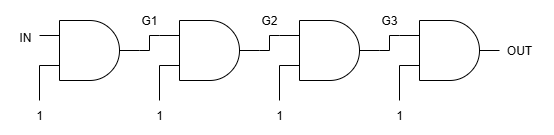
\includegraphics[width=0.7\linewidth]{picture/E2.png}
    \caption{AND回路4段の遅延を測定する回路}
    \label{E2}
\end{figure}

この回路では、「2入力AND回路の片方の入力値が1のとき、出力値はもう片方の入力値と同じになる」ことを用いて、INから入力された値をそのままOUTから出力することができる。
図\ref{E2}の回路において、入力INに方形波を与えることを考える。方形波の周期がAND回路4段分の遅延に比べて十分に長い(つまり、周波数が十分に低い)とすると、図\ref{E2}における各信号IN, G1, G2, G3, OUTの波形は図\ref{E3}のようになる。なお、図\ref{E3}において、$T$はAND回路1個当たりの遅延時間を表している。
オシロスコープで、INとOUTの電圧波形の時間軸上のずれを測定できれば、AND回路1個分の遅延の4倍に相当する$4T$を知ることができる。
\begin{figure}[htbp]
    \centering
    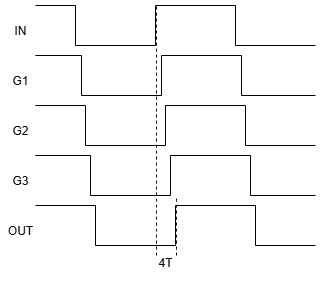
\includegraphics[width=0.7\linewidth]{picture/E3.png}
    \caption{図\ref{E2}の入力に方形波を入力したときの信号の伝搬}
    \label{E3}
\end{figure}

\subsection{使用機器}
USBコンセント, 信号発生器, AND回路 SN74HC08N 3個, オシロスコープ, ブレッドボード
\begin{figure}[htbp]
    \centering
    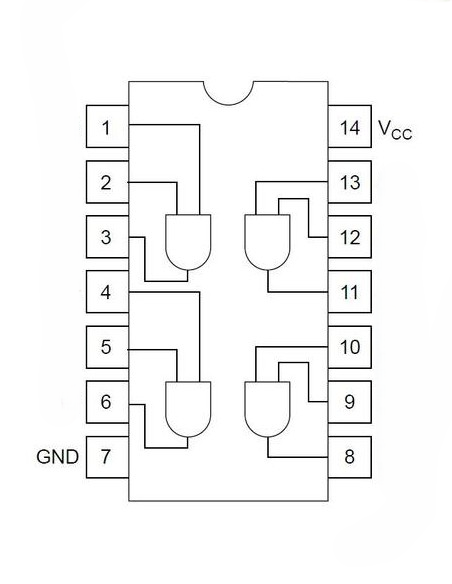
\includegraphics[width=0.5\linewidth]{picture/E4.png}
    \caption{SN74HC08Nの端子配置と内部論理回路図}
    \label{E4}
\end{figure}

\subsection{実験方法}
\subsubsection*{実験2-1 AND回路の遅延測定}
図\ref{E5}に示す回路をブレッドボード上に組み、電圧$v_0$が周波数\SI{1}{\kilo\hertz}、最小値\SI{0}{\volt}、最大値\SI{5}{\volt}の方形波となるように、オシロスコープで波形を確認しながら調整した。
配線の概略を図\ref{A1}に示す。
その後、電圧$v_1$と$v_2$の時間差が分かるようにオシロスコープ上に波形を表示して、時間差を記録し、加えて、その画像を保存した。
図\ref{O9}にその画像を示す。

図\ref{O9}より、$v_1$と$v_2$の測定された時間の差は約\SI{13}{\nano\second}と分かる。
そこから、AND回路1個あたりの遅延を求めると、約\SI{3.25}{\nano\second}と分かる。
\begin{figure}[htbp]
    \centering
    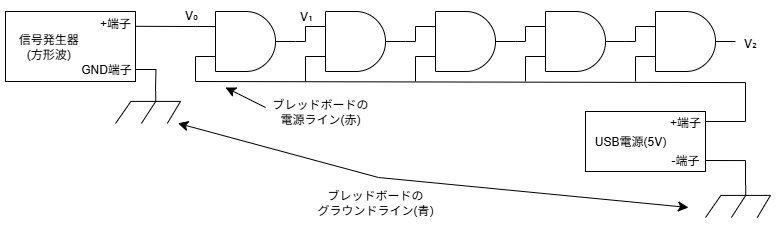
\includegraphics[width=0.7\linewidth]{picture/E5.png}
    \caption{実験回路2}
    \label{E5}
\end{figure}
\begin{figure}[htbp]
    \centering
    \includegraphics[width=0.7\linewidth]{picture/A1.png}
    \caption{作成した配線の下書き}
    \label{A1}
\end{figure}
\begin{figure}[htbp]
    \centering
    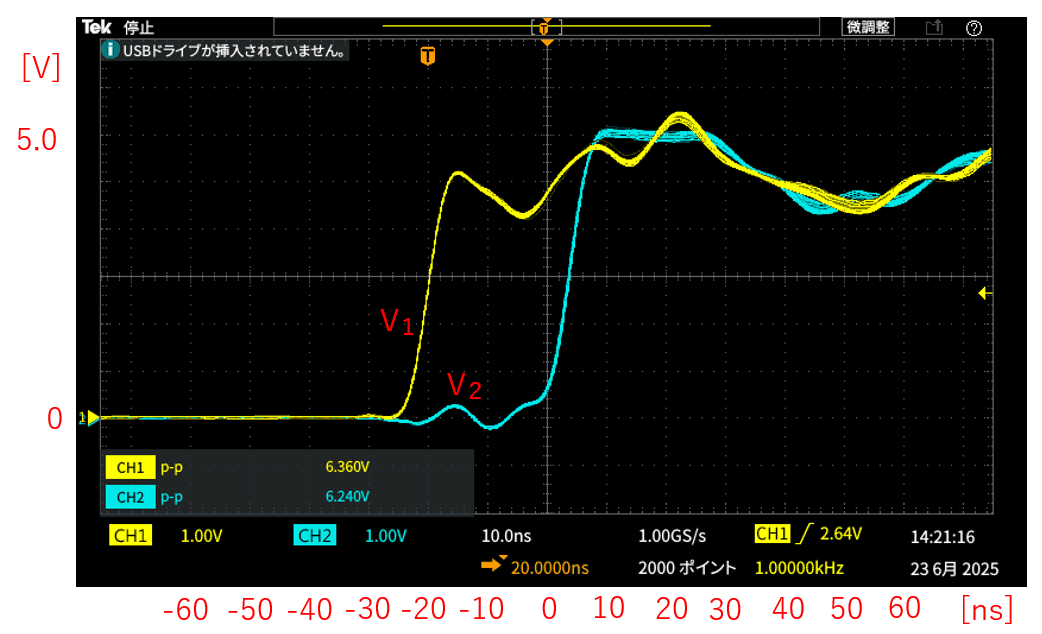
\includegraphics[width=0.8\linewidth]{picture/O9.png}
    \caption{図\ref{E5}の回路の$v_1$,$v_2$の電圧の波形}
    \label{O9}
\end{figure}

\subsubsection*{実験2-2 ファンアウト数と遅延の関係の測定}
ファンアウト数とは、論理素子の出力が、いくつの論理素子の入力として使われているかを表す数である。
ファンアウト数が1, 2, 3の例を図\ref{E6}に示す。
\begin{figure}[htbp]
    \centering
    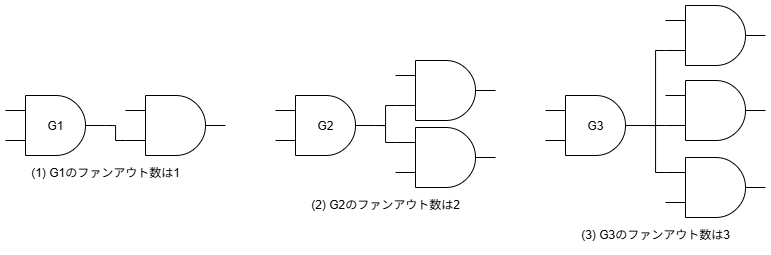
\includegraphics[width=0.7\linewidth]{picture/E6.png}
    \caption{ファンアウト数}
    \label{E6}
\end{figure}

実験2-1で作った回路のうち、方形波を生成する部分はそのままにして、論理回路部分のみを図\ref{E7}に変更し、実験2-1と同様に、電圧$v_0$が周波数\SI{1}{\kilo\hertz}、最小値\SI{0}{\volt}、最大値\SI{5}{\volt}の波形になるように調整し、オシロスコープで$v_1$と$v_2$の時間差を測定した。その結果を図\ref{O10}に示す。
続いて、図中のL1, L2, L3, L4を1つずつ外していった場合の遅延を測定し、どのような変化があるかを確認した。
それぞれの波形を図\ref{O11-14}に示す。


図\ref{O10}より、$v_1$と$v_2$の測定された時間の差は約\SI{15.5}{\nano\second}と分かる。
また図\ref{O11-14}より、ファンアウト数が減るごとに$v_1$と$v_2$の時間差、つまり遅延時間が短くなっていることが分かる。
\begin{figure}[htbp]
    \centering
    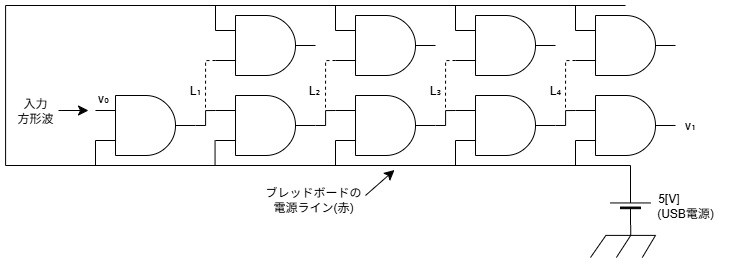
\includegraphics[width=0.7\linewidth]{picture/E7.png}
    \caption{実験回路3}
    \label{E7}
\end{figure}
\begin{figure}[htbp]
    \centering
    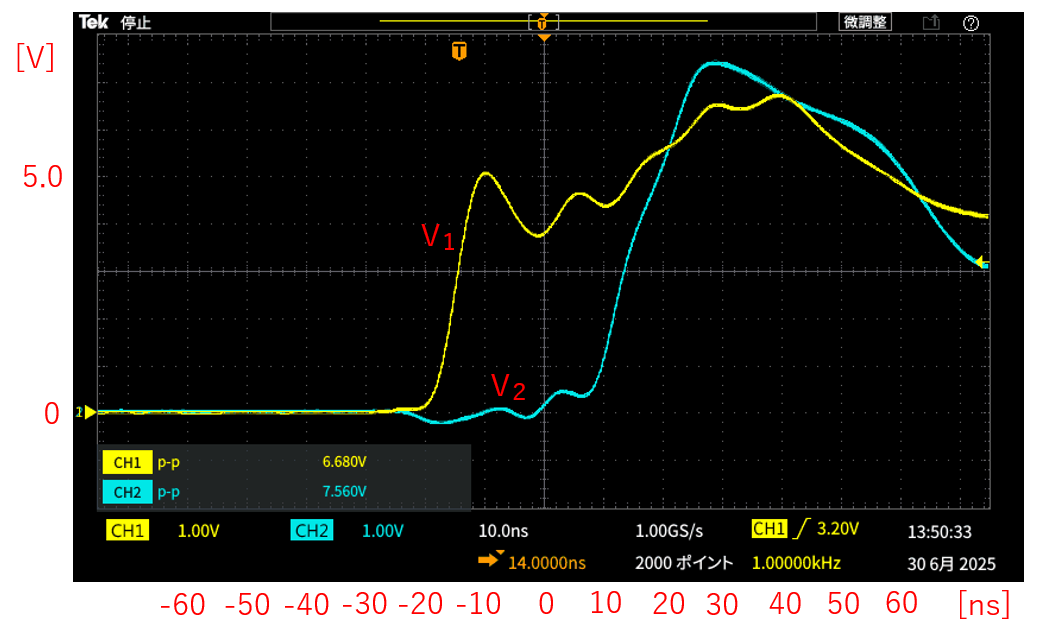
\includegraphics[width=0.8\linewidth]{picture/O10.png}
    \caption{図\ref{E7}の回路の$v_1$,$v_2$の電圧の波形}
    \label{O10}
\end{figure}

\begin{figure}[htbp]
    \centering
    \begin{subfigure}[b]{0.48\textwidth}
        \centering
        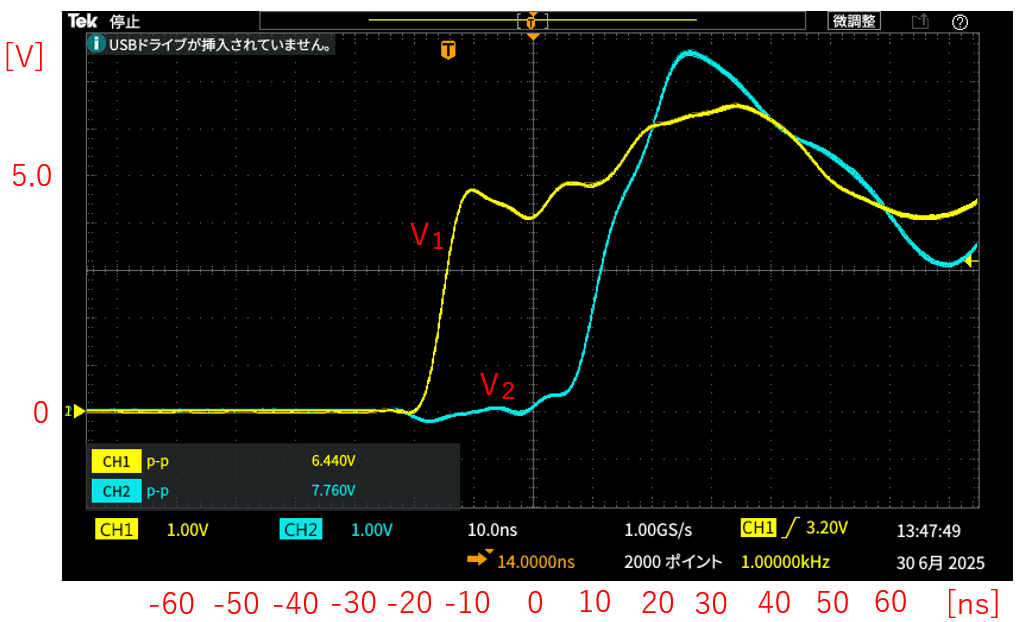
\includegraphics[width=\linewidth]{picture/O11.png}
        \caption{ファンアウト数が3のとき}
        \label{O11}
    \end{subfigure}
    \hfill
    \begin{subfigure}[b]{0.48\textwidth}
        \centering
        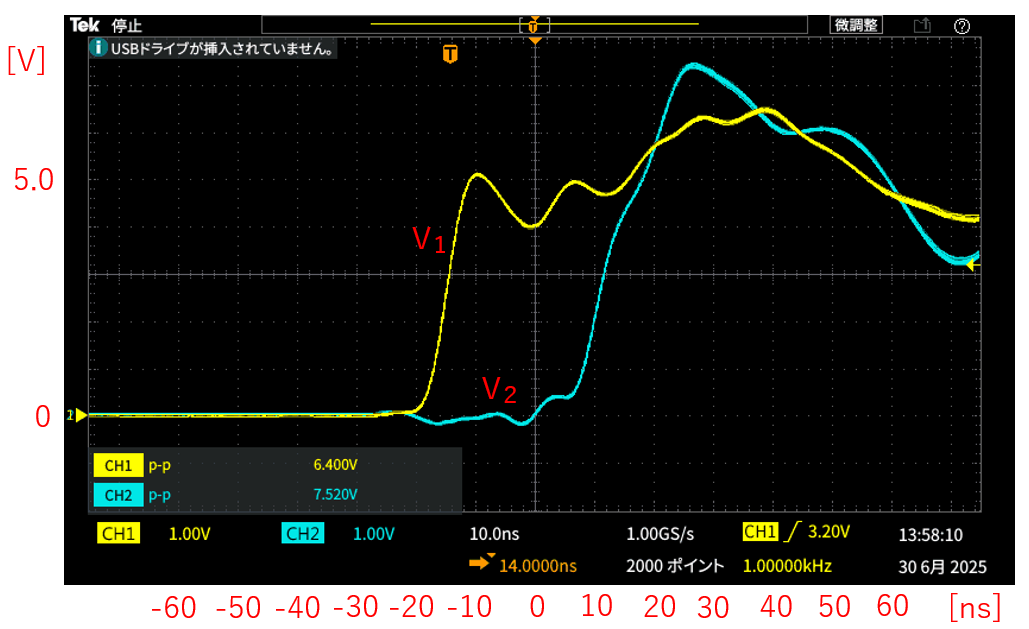
\includegraphics[width=\linewidth]{picture/O12.png}
        \caption{ファンアウト数が2のとき}
        \label{O12}
    \end{subfigure}
    
    \vspace{1ex}
    
    \begin{subfigure}[b]{0.48\textwidth}
        \centering
        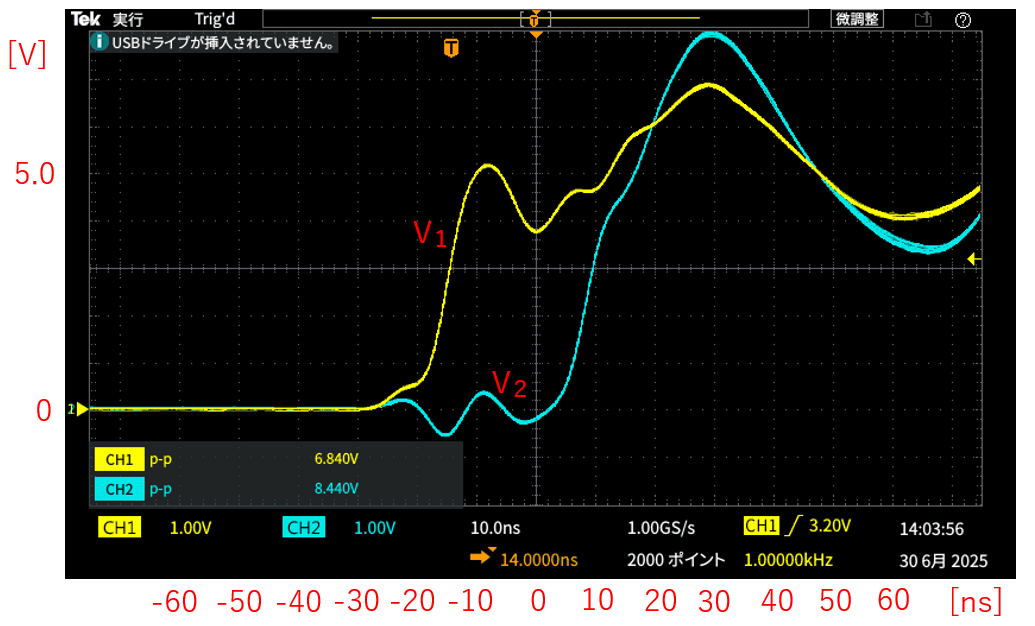
\includegraphics[width=\linewidth]{picture/O13.png}
        \caption{ファンアウト数が1のとき}
        \label{O13}
    \end{subfigure}
    \hfill
    \begin{subfigure}[b]{0.48\textwidth}
        \centering
        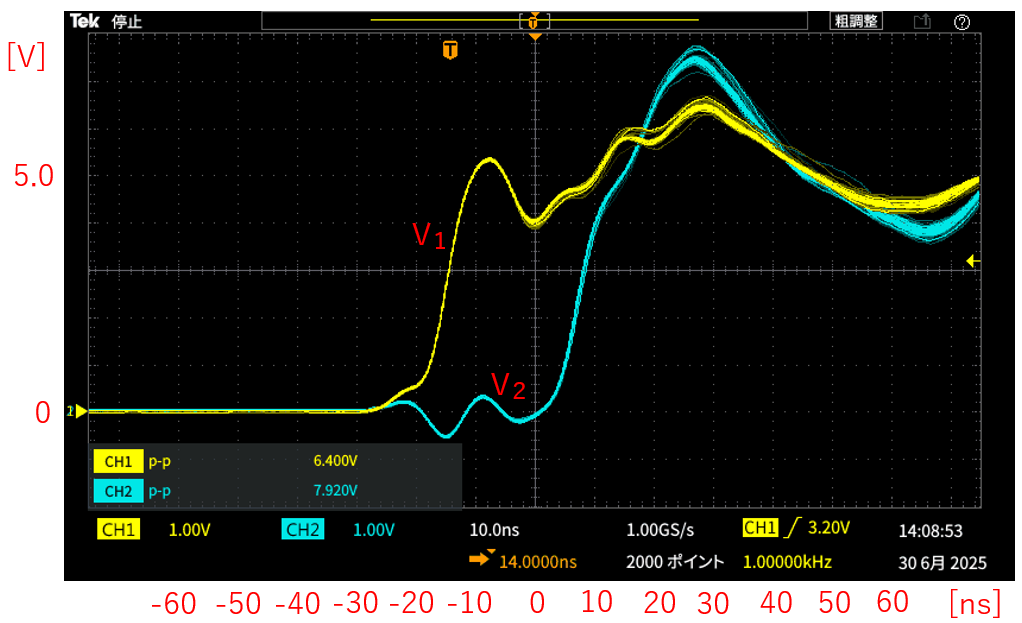
\includegraphics[width=\linewidth]{picture/O14.png}
        \caption{ファンアウト数が0のとき}
        \label{O14}
    \end{subfigure}
    \caption{実験2-2 ファンアウト数と遅延の関係}
    \label{O11-14}
\end{figure}

\clearpage

\subsection{考察課題}
\begin{enumerate}[label=(\arabic*), itemsep=1.5ex, leftmargin=2.5em]
    \item 2入力AND回路の片方の入力値が1のとき、出力値はもう片方の入力値と同じになる。2入力AND回路は、2つの入力がともに1のときのみ、出力が1となる論理回路である。そのため、片方の入力を1にしたとき、もう片方が0なら出力は0に、1なら出力は1となる。よって、2入力AND回路の片方の入力値が1のとき、出力値はもう片方の入力値と同じになっていることが分かる。
    
    \item この実験でのAND回路の遅延測定と同様に、4段の論理素子の遅延を測定して求める方法で、OR, NAND, NORの遅延を図るとする。実験2-1より、論理素子を4段接続する場合は、入力信号と同じ値を出力する必要があると考えられる。
    OR回路の場合は、2入力OR回路を4段接続し、一方の入力端子から方形波を入力し、もう一方の入力端子はすべてを0に固定することで測定できる。
    NAND回路の場合は、2入力NAND回路を4段接続し、一方の入力端子から方形波を入力し、もう一方の入力端子はすべてを1に固定することで測定できる。
    NOR回路の場合は、2入力NOR回路を4段接続し、一方の入力端子から方形波を入力し、もう一方の入力端子はすべてを0に固定することで測定できる。
    
    \item 実験2-1では、AND回路1個当たりの遅延時間は約\SI{3.25}{\nano\second}であるという結果が得られた。しかし、実験に用いたAND回路のデータシートを確認すると、今回と同じ似た条件での平均遅延時間は約\SI{8}{\nano\second}であることが分かった。遅延時間がデータシートよりも短い結果となったのは、ICの個体差や測定方法の誤差、データシートとの測定条件(電源電圧、温度、負荷容量)の相違などが考えられる。
\end{enumerate}

\section{記憶素子の作成と測定}
\subsection{原理}
図\ref{E8}は、2つのNOT回路を接続し、その入力と出力をリング状に接続させた回路である。
NOT回路は、入力値の否定が出力値となるため、2段接続した場合、「否定の否定」となるため、図の右側か左側のどちらかの状態になって安定する(どちらの状態になるかは、電源を入れてみないと分からないし、その時々で変わる可能性もある)。
このように、「否定の否定は元の値に戻る」を利用して、図\ref{E8}のように同じ値を保ち続けることが、値を記憶する原理の基本となる。なお、図\ref{E8}は図\ref{E9}のように示されることもあるが、これらは全く同じ回路である。
\begin{figure}[htbp]
    \centering
    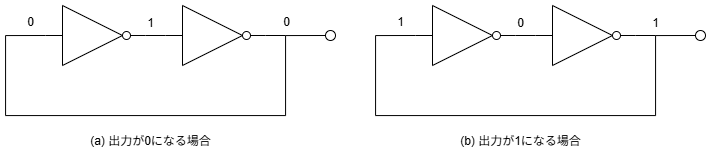
\includegraphics[width=0.7\linewidth]{picture/E8.png}
    \caption{NOT回路の2段接続した回路}
    \label{E8}
\end{figure}
\begin{figure}[htbp]
    \centering
    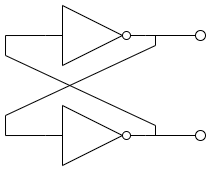
\includegraphics[width=0.5\linewidth]{picture/E9.png}
    \caption{図\ref{E8}と等価な回路の別の描き方}
    \label{E9}
\end{figure}

次に、図\ref{E10}の回路について考える。この回路はRSラッチと呼ばれる回路であり、2つの入力端子SとRを持つ。
以下、入力値の全ての組み合わせについて、回路がどのような動作をするか解説する。
\begin{itemize}
    \item \textbf{S=1, R=0のとき}
    NOT回路により、S'=0, R'=1となる。NAND回路はAND回路の否定であるから、片方の入力が0であれば出力が1になるため、Q=1となる。Q=1, R'=1より、QB=0となる。

    \item \textbf{S=0, R=1のとき}
    NOT回路により、S'=1, R'=0となる。NAND回路の片方の入力が0であれば出力は1になるため、QB=1となる。QB=1, S'=1より、Q=0となる。

    \item \textbf{S=0, R=0のとき}
    図\ref{E11}にしめすように、NAND回路の片方の入力が1の場合、他方の入力の否定が出力となる。そのため、S=0,R=0のときは、S'=1,R'=1となるため、図\ref{E9}に示したNOT回路を接続した回路と等価になる。そのため、S=0,R=0になる直前のQ,QBの値がそのまま変わらずに出力される。ただし、電源を入れた時にS=0,R=0である場合には、Qの値が1になるか0になるかは分からない。

    \item \textbf{S=1, R=1のとき}
    NOT回路により、S'=0,R'=0となる。よって、NAND回路の出力Q,QBはともに1になる。
\end{itemize}
\begin{figure}[htbp]
    \centering
    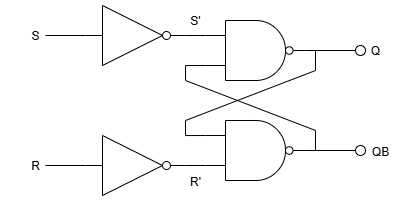
\includegraphics[width=0.7\linewidth]{picture/E10.png}
    \caption{RSラッチ回路}
    \label{E10}
\end{figure}
\begin{figure}[htbp]
    \centering
    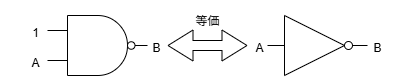
\includegraphics[width=0.7\linewidth]{picture/E11.png}
    \caption{NAND回路の片方の入力が1の場合、NOT回路と等価である}
    \label{E11}
\end{figure}

以上をまとめると、RSラッチの状態の変化は表\ref{H1}のようにまとめることができる。
この回路は、次の意味で、値を記憶することができる回路である。
\begin{itemize}
    \item (R=0の間は)S=1にするとQ=1になり、その後、Sが1であろうと0であろうとQ=1を記憶することができる
    \item (S=0の間は)R=1にするとQ=0になり、その後、Rが1であろうと0であろうとQ=0を記憶することができる
\end{itemize}
なお、S=1,R=1は禁止されている入力であり、RSラッチにこの入力を与えてはいけないことになっている。

\begin{table}[htbp]
    \centering
    \caption{RSラッチの動作}
    \label{H1}
    \begin{tblr}{
      colspec = {|c|c|},
      hlines,
      vlines
    }
        入力 & 次の $Q, QB$ の値 \\
        \hline
        $S=0,R=0$ & $Q,QB$ の値は変わらない \\
        $S=1,R=0$ & $Q=1,QB=0$ \\
        $S=0,R=1$ & $Q=0,QB=1$ \\
        $S=1,R=1$(禁止入力) & $Q=1,QB=1$ \\
    \end{tblr}
\end{table}

\subsection{使用機器}
USBコンセント(NAND回路の電源用), 直流安定化電源(入力SとRの電圧用), NAND回路 SN74HC00N 1個, LED 2個, 抵抗器(\SI{200}{\ohm})2個, ブレッドボード

\subsection{実験方法}
\subsubsection*{実験3 RSラッチの測定}
図\ref{E12}に示す回路をブレッドボード上に組み、入力RとSの電圧を表\ref{H2}に記されているように与えた。
そのときのLED点灯状況を見て、出力QとQBの値が0か1かを表\ref{H2}に示す。
なお、この実験では、RSラッチの出力Q,QBの値はLEDの点灯で確認することができ、出力QにつないだLEDが点灯しているときはQ=1、消灯しているときはQ=0である。出力QBについても同様である。

表\ref{H2}により、最後に\SI{5}{\volt}にしたAND回路側のLEDが点灯していることが分かる。
\begin{figure}[htbp]
    \centering
    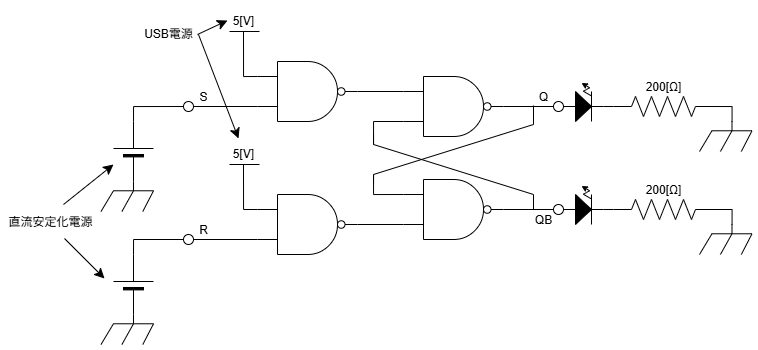
\includegraphics[width=0.7\linewidth]{picture/E12.png}
    \caption{RSラッチ実験回路}
    \label{E12}
\end{figure}

\begin{table}[htbp]
    \centering
    \caption{LED点灯状況の記録表}
    \label{H2}
    \begin{tblr}{
      colspec = {|c|*{8}{c|}},
      hlines
    }
    欄 & A & B & C & D & E & F & G & H \\
    {電圧(S) \\ (\si{\volt})} & 0 & 0 & 0 & 5 & {0〜5で\\任意に変化} & 0 & 0 & 5 \\
    {電圧(R) \\ (\si{\volt})} & 0 & 5 & 0 & 0 & 0 & 5 & {0〜5で\\任意に変化} & 5 \\
    $Q$  & 1 & 0 & 0 & 1 & 1 & 0 & 0 & 1 \\
    $QB$ & 0 & 1 & 1 & 0 & 0 & 1 & 0 & 1 \\
    \end{tblr}
\end{table}

\subsection{考察課題}
\begin{enumerate}[label=(\arabic*), itemsep=1.5ex, leftmargin=2.5em]
    \item 図\ref{E12}で用いたRSラッチ回路は、図\ref{E10}のものと同じである。図\ref{E10}の回路では、2つの入力はNOT回路を通り、2つのNAND回路を交差するように通る。図\ref{E11}の回路のより、NAND回路の片方の入力が1の場合、NOT回路と等価となるため、図\ref{E10}の回路の片方の入力を1に固定すると、もう片方の値の逆を出力するNOT回路となる。図\ref{E12}の回路では、2つの入力はそれぞれ別のNAND回路を通った後、2つのNAND回路を交差するように通る。これも同様に処理すると、図\ref{E10}と同じように、片方の値の逆を出力するNOT回路となる。よって、2つの回路は同じものとなる。

    \item 表\ref{H2}の結果より、図\ref{E12}のRSラッチ回路を上下で分けた時、直前に入力で\SI{5}{\volt}を与えた側の回路部分に\SI{5}{\volt}の電圧を出力する回路であると考えられる。また、入力を与えていないときはどちらかの回路部分に出力されると分かる。
    
    \item スイッチのON/OFFを切り替える際に「チャタリング」という現象が生じる。チャタリングとは、スイッチ内部の金属接点が、接触する瞬間に物理的に微細なバウンドを繰り返し、断続的に接触してしまうことである。つまり、スイッチがON/OFFを高速に繰り返し、意図していない動作を繰り返すという現象である。チャタリングは、RSラッチを用いることで取り除くことができる。RSラッチは最初の入力が入った時点でその状態を保存するため、金属接点がバウンドによって、ON/OFFを高速に繰り返すのを完全に無視して、安定した動作をすることが可能であるからである。
\end{enumerate}

\section{感想}
今回の実験を通して、論理素子の使い方やその動作における遅延についてや、ディジタル回路において値を記憶する回路の構成についてを知ることができた。
また、実際に回路を作成し、出力を測定し、読み取る力をつけることもできた。
今後、ディジタル回路を作成する機会があった際は、実験を通しての検証もしていき、より一層理解を深めていきたいと思う。

\section{参考文献}
\begin{thebibliography}{9}

    \bibitem{ref1}
    エンジャー, 『オシロスコープの基本\&使い方』,
    \url{https://engineer-climb.com/osc-basic/}, 2025年7月21日閲覧.

    \bibitem{ref2}
    横河計測株式会社, 『プローブの基礎』, 
    \url{https://tmi.yokogawa.com/jp/library/resources/measurement-tips/probe_basics/}, 
    2025年7月21日閲覧.

    \bibitem{ref3}
    エンジニアの電気屋さん, 『AC結合とDC結合の違いをオシロスコープで確認してみた』,
    \url{https://misoji-engineer.com/archives/ac-dc-coupling.html}, 
    2025年7月21日閲覧.

    \bibitem{ref4}
    東芝デバイス\&ストレージ, 『データシートの見方』,
    \url{https://toshiba.semicon-storage.com/jp/semiconductor/knowledge/e-learning/cmos-logic-basics/chap4/chap4-3-1.html}, 2025年7月21日閲覧.

    \bibitem{ref5}
    パープルハット, 『NANDだけでNOT・AND・OR回路を作成』,
    \url{https://kiironomidori.hatenablog.com/entry/nand-not-and-or}, 2025年7月21日閲覧.

    \bibitem{ref6}
    marutsu, 『スイッチのチャタリングの概要。チャタリングを防止する方法。』,
    \url{https://www.marutsu.co.jp/pc/static/large_order/1405_311_ph}, 2025年7月21日閲覧.
\end{thebibliography}

\end{document}